\documentclass{article}

% Language setting
% Replace `english' with e.g. `spanish' to change the document language
\usepackage[english]{babel}

% Set page size and margins
% Replace `letterpaper' with `a4paper' for UK/EU standard size
\usepackage[letterpaper,top=2cm,bottom=2cm,left=3cm,right=3cm,marginparwidth=1.75cm]{geometry}

% Useful packages
\usepackage{amsmath}
\usepackage{graphicx}
\usepackage[colorlinks=true, allcolors=blue]{hyperref}
\usepackage{tikz}
\usetikzlibrary{shapes.arrows, positioning, arrows.meta}


\title{Theoretical framework}
\author{Riccardo Dal Cero}

\begin{document}
\maketitle

\begin{abstract}
    The main idea is to study how and whether the asymmetry of information have an impact on the cleansing effect of
    recession, replicating the model in computer  simulation.
\end{abstract}

\section[short]{Theoretical framework}
The economy consists of firms that are risk-neutral and have a constant discount rate represented by the parameter $0 <
\beta < 1$. These firms exhibit heterogeneity in terms of their productivity and net worth. They utilize a production
technology that takes capital (or production units) as the sole input, with diminishing returns to scale. 
\par
In each period, firms incur a fixed production cost denoted as $c$ to initiate production. Following production, firms
make decisions regarding the allocation of profits for the next period. The remaining portion of profits is invested in
a risk-free asset. Firms face a choice: they can either remain in the market and reinvest their profits or exit the
market entirely, investing their entire net worth, denoted as $e$, in the risk-free asset. 
\par
When firms choose to exit the market, they forgo any future profits, but they also free themselves from the financial
burden of the fixed cost represented by $c$. Consequently, firms opt to exit the market when the expected profits fail
to outweigh the fixed cost, or when the value of production becomes inferior to the value they could gain by investing
in the risk-free asset.
\par
This value, obtained from investing in the risk-free asset, is equal to $q_t +
\sum_{s=0}^{+\infty}\beta^s[\beta(1+r)-1]e_{t+s+1}$. Notably, when the condition $\beta(1+r) \leq 1$ holds true, this
value simplifies to $q$. In such cases, firms are either indifferent regarding the timing of dividend distributions or
have a preference for distributing their end-of-period net worth to shareholders or investors.

\par
The agents in this economy are the firms themselves, and they aim to maximize their value over time by selecting an
optimal level of capital denoted as $k$. The production function, after accounting for the fixed cost $c$, can be
expressed as follows: $Y = Z(\theta + \epsilon)k^\alpha$.
\begin{itemize}
    \item $Z$: is the stochastic aggregate productivity common across firms 
    \item $\theta$: is a persistent firm-specific productivity shock (model as a Markov Chain)     
    \item $\epsilon$: is the firm-specific productivity shock $\epsilon\sim\mathcal{N}(0,\sigma ) $
    \item $k^\alpha$: capital or production units as in (Caballero Hammour, AER)
\end{itemize}
The timeline of the events is the following
\begin{figure}[h]
    \centering
    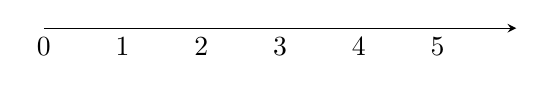
\begin{tikzpicture}
        % Draw timeline
        \draw[->,>=stealth] (0,0) -- (6,0);
        
        % Add timeline labels
        \foreach \x/\label in {0,1, 2,3, 4, 5} {
            \node[align=center, below] at (\x,0) {\label};
        }
        
        
    \end{tikzpicture}
    \caption{Timeline of Events}
\end{figure}
\begin{enumerate}
    \item firm knows \(Z,\theta,k^\alpha,e\) where $e$ is its endowment\footnote{which is different from $k$ since the
    firm can borrow money: \(d=c+k-e\) where $d$ stays for debt} 
    \item firm compute the $k$ need to maximizes the expected value of the firm range can varies from \([0,+\infty]\) if
    $k=0$ it means that the firm decide to exit.
    \item at the end of the period the firm observe \(\epsilon_{t}\) and the aggregate shock
    \item repays its debt and the fixed operating cost \(c+k-e\), the firm its left with the end of period net worth $q$
    \item decide the amount the dividend to distribute \(q-e_{t+1}\) observe the productivity shock \(\theta_{t+1},
    Z_{t+1}\) and the step restart from 1
\end{enumerate}
\subsection{Frictionless economy}
In a frictionless economy, firms have the option to borrow an amount denoted as \(c+k-e\) at the risk-free interest rate
\(r=\frac{1}{\beta}-1\). Therefore, at the start of the period, the firm's value is determined by the following
expression:

\[V_{FL} = \max_{k} E \int \max[q,\max_{e_{t+1}}(q - e_{t+1} + \beta V_{FL}(e_{t+1},\theta_{t+1}, Z_{t+1}))]  \,d\Phi
(\epsilon) \]
where the end of period net worth is equal to:
\[q=Z(\theta+\epsilon)k^\alpha + (1-\delta )k-(1+r)(c+k-e)\]

Under the condition of survival, it can be demonstrated that:

\[\widehat{V}_{FL}(\theta,Z) = \max_{k}E\int[Z(\theta+\epsilon)k^\alpha - (1+r)c\,d\Phi (\epsilon)] +
\beta\max[0,\widehat{V}_{FL}(\theta_{t+1},Z_{t+1})]\]

In the absence of market frictions, firms choose to exit when their productivity reaches a certain threshold.
Specifically, they exit if \(\theta_{t+1}<\underline{\theta} _{FL}(Z_{t+1})\), where \(\underline{\theta}
_{FL}(Z_{t+1})\) is defined as the value
for which \(\widehat{V}_{FL}(\underline{\theta}_{FL},Z_{t+1})=0\).

\subsection{The economy with credit market frictions}
After the production the transitory shock \(\epsilon\) is privately observed by the firm, whereas the financial
intermediaries can observe only at cost \(\mu k^\alpha\). Considering one period debt contract the financial
intermediary observe \(\epsilon\) only if the firm fails, thus when the private shock is not enough to repays its debt.
The terms of the financial contract depends on the value of the firm's net worth\(e\), on its current productivity \(\theta\), and on the value of
aggregate productivity \(Z\), all observable by the financial intermediary and the firm at zero
cost. 
\par
HP1: The risk-free interest rate is \(\beta<\frac{1}{1+r}\) \\
Thus the risk-free rate is lower in an economy with credit frictions than in the frictionless one, and garantess  that
firm do not always reinvest their profits.
When a firm is not able to reimburse its debt,
it defaults. In this case, the financial intermediary pays a cost to verify the firm's income
and confiscates all the firm's income. The default threshold \(\overline{\epsilon} \)is given by:
\[Z(\theta+\overline{\epsilon} )k^\alpha +(1-\sigma)k = (1+r)(c+k+e)\]
Default leads to a zero net worth but does not necessarily lead to the exit of the firm
as observed empirically. Depending on its persistent productivity component \(\theta\), the firm
could find profitable to stay in the market with zero net worth.
The financial intermediary lends (c + k -e) to the firm only if its expected income from
the loan is equal to the opportunity cost of the funds. 
\[(1+r)(k+c+e)(1-\Phi(\overline{\epsilon}))+\int_{-\infty}^{\overline{\epsilon}}[Z(\theta+\overline{\epsilon} )k^\alpha
+(1-\sigma)k-mu k^\alpha]  \,d\Phi(\epsilon)\geq (1+r)(c+k+e) \]

\end{document}